The second software that has been worked on is a Particle Jet Substructure Adversarial Neural Network, and is discussed in further detail in chapters \ref{ch:jsann} and \ref{ch:analysisjsann}. This chapter aims to explain briefly what a Neural Network is, and the added complexity of it being an adversarial one.

\section{What is a neural network?}

Neural networks are a biologically influenced model, with the aim to learn, recognise patterns, and make decisions in a human-like way. They are used in various applications, ranging from stock market prediction to medical science \cite{ch7nn} and rely on a plain and systematic way of analysing input data. They have achieved considerable success due to today’s recently data availability growth and affordable computational power \cite{nnarticle1}.

%\begin{figure}[H]
%    \centering
\begin{figure}]H]%{0.48\textwidth}
  \centering
  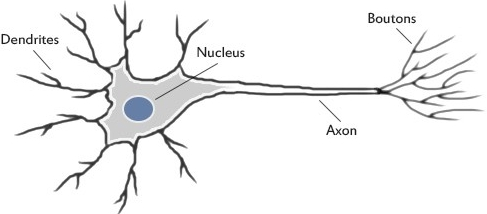
\includegraphics[width=1\textwidth]{images/nn0.jpeg}
  \caption{A neuron in our brain. From \cite{nnarticle2}.}
  \label{fig:realnneuron}
\end{figure}

The human brain uses a network of neurons to process information and model the world around us. A neuron (shown in figure \ref{fig:realnneuron}) collects inputs from other neurons, using dendrites, and sums them. If the resulting value is greater than a threshold, it fires; The signal is then sent to other nearby neurons in the network. 

\begin{figure}[H]%{0.48\textwidth}
  \centering
  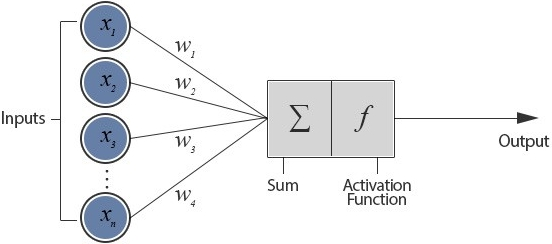
\includegraphics[width=1\textwidth]{images/nn1.jpeg}
  \caption{Model of an artificial neuron (Perceptron). From \cite{nnarticle2}.}
  \label{fig:artifialneuron}
\end{figure}
%\label{neurons}
%\caption{blah blah neurons. From \cite{nnarticle2}}
%\end{figure}


Artificial neural networks mimic that behaviour. As can be seen in figure \ref{fig:artifialneuron}, a neuron is connected with a number of other neurons and receives inputs from them. This configuration is called a Perceptron. 

All the inputs are individually weighted, added together and passed into an activation function. The inputs ($x_i$) and weights ($w_i$) are real numbers and can be positive or negative. The purpose of the activation function is to transform the input signal into an output signal and are necessary for neural networks to model complex non-linear patterns that simpler models might miss. There are many types of activation functions: linear, sigmoid, hyperbolic tangent and more. 

\begin{comment}
There are various options for an activation function but the simplest one is the step function\footnote{A step function will typically output a 1 if the input is higher than a certain threshold, otherwise it’s output will be 0.}.

An example\cite{nnarticle2} would be,
\begin{itemize}[noitemsep]
    \item[] Input 1 ($x_1$) = 0.6, Input 2 ($x_2$) = 1.0
    \item[] 
\end{itemize}
\begin{itemize}[noitemsep]
    \item[] Weight 1 ($w_1$) = 0.5
    \item[] Weight 2 ($w_2$) = 0.8
\end{itemize}
\begin{itemize}[noitemsep]
    \item[] Threshold = 1.0 
\end{itemize}
Weighing the inputs and adding them together gives, 
\begin{itemize}[noitemsep]
\item[]$x_1 * w_1 + x_2 * w_2 = (0.6 * 0.5) + (1 * 0.8) = 1.1$
\end{itemize}

Here, the total input is higher than the threshold and thus the neuron fires. 
\end{comment}

A neural network is created by assembling together many simple perceptrons, so that the output of one of them can be the input of another. For example, figure \ref{fig:simplerernn} shows a small neural network. In this example, the three main parts of a neural network can be identified: the input layer (layer 1), the hidden layer (layer 2), and the output layer (layer 3). The input layer consists of as many perceptrons as there are variables in the input data, while the output layer of as many as the output of the neural network is. The hidden layer is responsible to transform the input data in a way that the output layer can use to reach conclusions.


\begin{figure}[H]
  \centering
  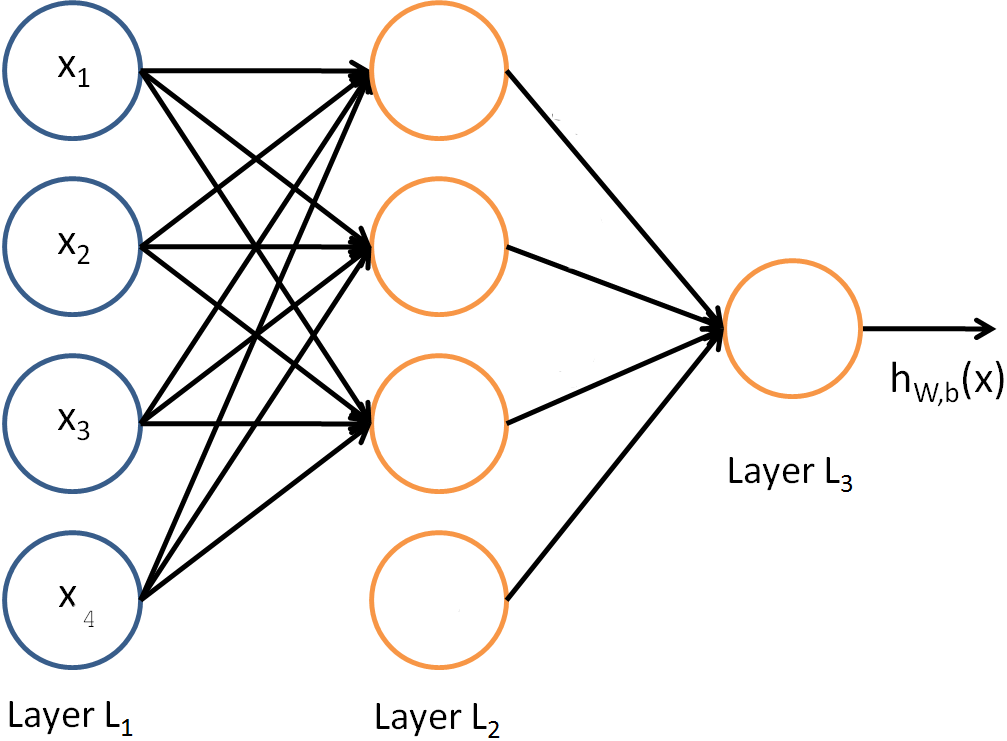
\includegraphics[width=\textwidth]{images/mysimplerernn.png}
  \caption{blah blah blah Taken from \cite{nnarticle3}}
  \label{fig:simplerernn}
\end{figure}

The circles represent neurons and lines represent synapses. Synapses take the input and multiply it by a “weight” (the “strength” of the input in determining the output). 

\section{Training a Neural Network}

For supervised training of a neural network, there should exist training data that have already been classified. This means that for every training input sample, the desired result of the neural network is known. 

The training involves calibrating all of the individual “weights” by repeating two key steps: forward propagation and back propagation. In forward propagation, a set of weights is being applied to the input data and the output is calculated. For the first forward propagation, the set of weights is selected randomly. In back propagation, the margin of error of the output is measured and the weights are adjusted accordingly to decrease the error using an equation.  This equation makes use of a lot of matrix vector multiplications.

Neural networks repeat forward and back propagation until the weights are calibrated to accurately predict an output. When all the training data have passed through the network, an epoch has passed, the network has (possibly) improved in predicting the correct output. Usually more than one epochs are needed for efficient training of the neural network. The loss function is a representative output of how many mistakes the neural network made during a training epoch.

\section{Using a Neural Network}
After the neural network has been trained, it can be used to make predictions in data it has not been trained on. Usually a part of the trained data are being reserved and not included in the training phase, so the neural network can be tested on them.

\section{Multi-layered neural networks}
\begin{figure}[H]
  \centering
  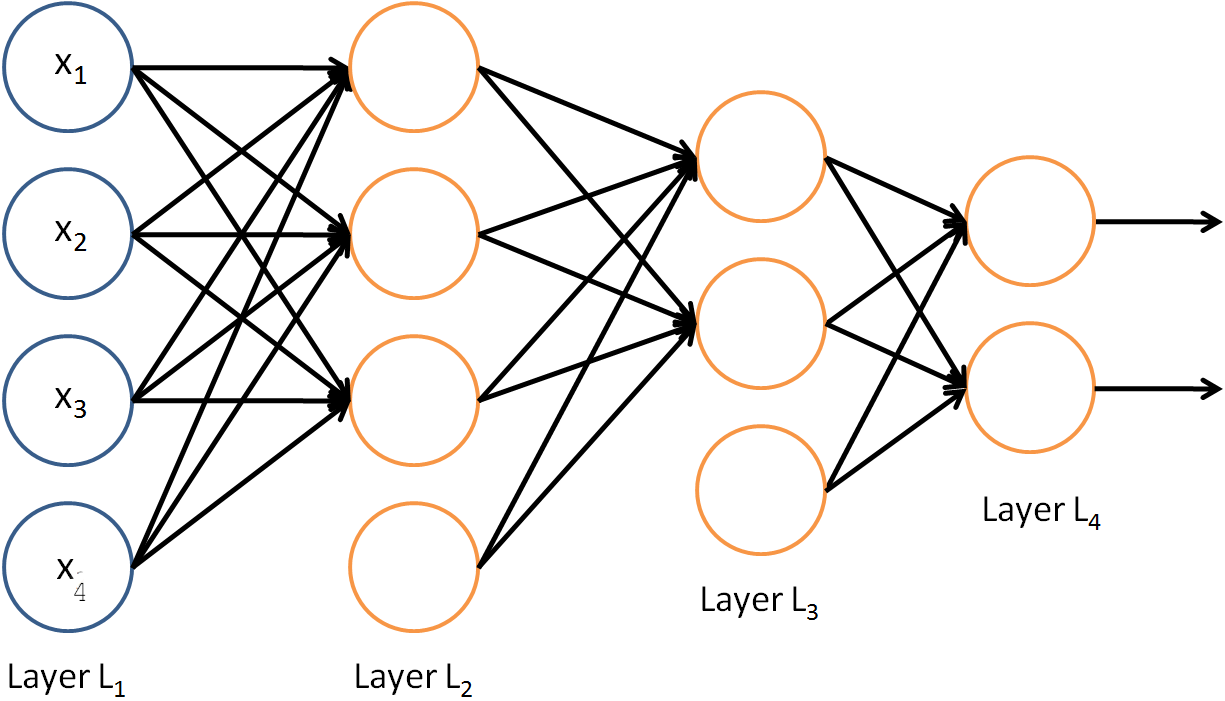
\includegraphics[width=\textwidth]{images/my_simplenn.png}
  \caption{blah blah blah Taken from \cite{nnarticle3}}
  \label{fig:simplenn}
\end{figure}

When the neural network has to make sense of something really complicated, more than one hidden layers are needed (figure \ref{fig:simplenn}) in order to transform the input data into information that the output layer can use to reach conclusions. The term “deep” learning came from having many hidden layers. 


\section{Adversarial Neural Networks}\label{ch:ann}
Adversarial Neural Networks is a recent idea \cite{goodfellow2014generative}, in which two models are trained simultaneously, competing with each other. 
%in a cat and mouse game. 
The first one is a generative model, that is a model whose task is to learn how to create new samples that are as close as possible to the input data.
The second model is what is called an adversary. The goal of the adversary is to determine whether a sample came from the input data or the generative model.

The two models are set in direct opposition. Generative model creates new samples and its adversary try to infer whether those came from the input data or the generative model. Both of them continuously improve from their interaction until a steady stage is reached.

%A generative model is set in direct opposition against an adversary: a discriminative model that learns to determine whether a sample is from the model distribution or the data distribution. 

The generative model can be thought of as analogous to a team of counterfeiters, trying to produce fake currency and use it without detection, while the adversary model is analogous to the police, trying to detect the counterfeit currency. Competition in this game drives both teams to improve their methods until the counterfeits are indistinguishable from the genuine articles \cite{goodfellow2014generative}.